\begin{frame}{SHACL — the constraint model (L2)}
  \framesubtitle{Shapes: what a valid instance must look like}

  \begin{columns}[T]
    \begin{column}{0.56\textwidth}
      \centering
      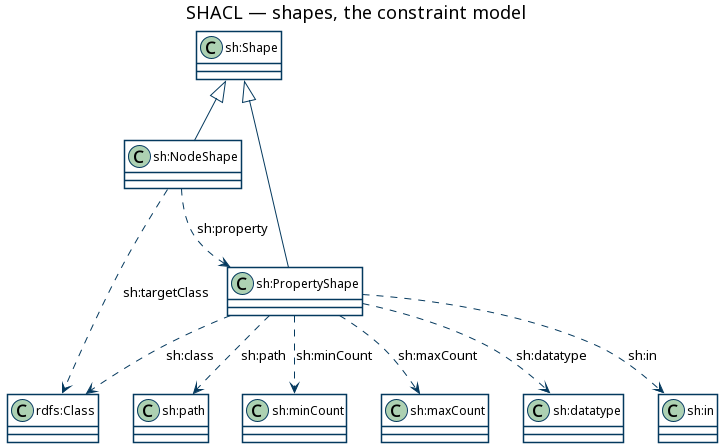
\includegraphics[width=\linewidth, height=0.6\textheight, keepaspectratio]{slides/im-101/shacl/figs/shacl.png}
    \end{column}
    \begin{column}{0.42\textwidth}
      \scriptsize
      \setlength{\itemsep}{0.5pt}
      \setlength{\parskip}{0pt}
      \textbf{Shapes}
      \begin{itemize}
        \item \texttt{sh:NodeShape} — constraints on a \emph{whole node}
        \item \texttt{sh:PropertyShape} — constraints on \emph{one property}
      \end{itemize}
      \vspace{0.4pt}
      \textbf{Targeting}
      \begin{itemize}
        \item \texttt{sh:targetClass} — which class the shape applies to
      \end{itemize}
      \vspace{0.4pt}
      \textbf{Property-shape constraints}
      \begin{itemize}
        \item \texttt{sh:in} — a closed value set
        \item \texttt{sh:datatype} — the value type
        \item \texttt{sh:minCount} / \texttt{sh:maxCount} — cardinality
        \item \texttt{sh:path} — which property
      \end{itemize}
      \vspace{2pt}
      \begin{alertblock}{}
        Closed world: what is missing \emph{means} something here.
      \end{alertblock}
    \end{column}
  \end{columns}
\end{frame}
